\chapter{Your Contribution}
\label{ch:ownwork}

Replace the chapter title above with a descriptive name for your main contribution. This is the core chapter of your thesis — it should present your approach, design, or system in enough detail that a reader could reproduce or build upon it.\footnote{If your contribution has multiple distinct components, consider splitting this into more than one chapter.}

%%%%%%%%%%%%%%%%%%%%%%%%%%%%%%%%%%%%%%%%%%%%%%%%%%%%%%%%%%%%%%%%%%%%%%%%
\section{Hypotheses}
\label{sec:hypotheses}

If your work is hypothesis-driven, state your hypotheses clearly here. For example:

\begin{itemize}
  \item[\textit{H1}] Your first hypothesis.
  \item[\textit{H2}] Your second hypothesis.
  \item[\textit{H3}] Your third hypothesis.
\end{itemize}

%%%%%%%%%%%%%%%%%%%%%%%%%%%%%%%%%%%%%%%%%%%%%%%%%%%%%%%%%%%%%%%%%%%%%%%%
\section{Approach}
\label{sec:approach}

Describe your approach, design, or methodology. Explain the decisions you made and justify them. Figures and tables should be used to support your explanation.

\subsection{Design}
\label{sec:design}

Describe the design of your system, study, or method. A figure is often the best way to convey an architecture or workflow:

\begin{figure}[ht]
  \centering
  % Replace with your own figure in the Images/ folder:
  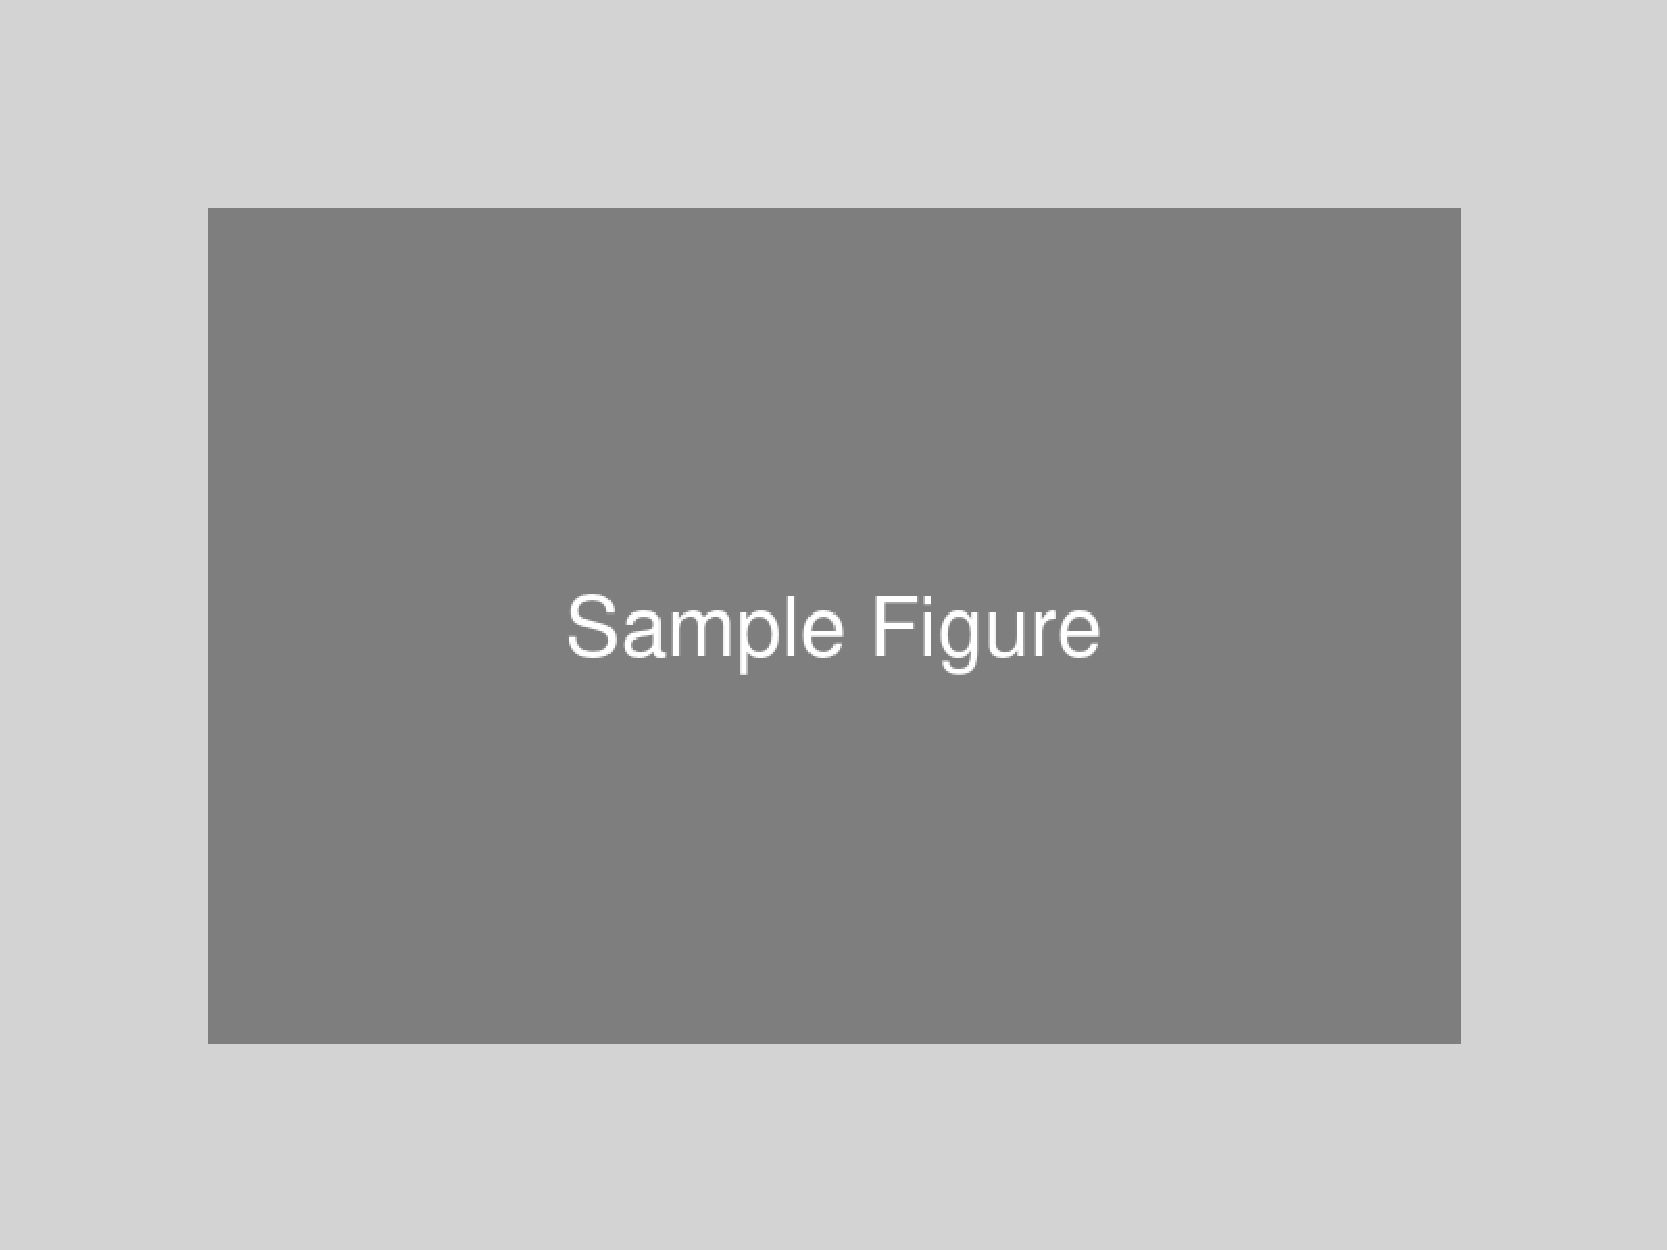
\includegraphics[width=0.8\textwidth]{images/sample-figure}
  \caption{A caption describing what the figure shows.}
  \label{fig:design}
\end{figure}

\subsection{Mathematical Formulation}
\label{sec:math}

If your approach involves a mathematical formulation, present it here. Use numbered equations for anything you refer to later in the text:

\begin{equation}
  f(x) = \frac{1}{\sigma\sqrt{2\pi}} \exp\left(-\frac{(x - \mu)^2}{2\sigma^2}\right)
  \label{eq:example}
\end{equation}

For multiple related equations, use the \texttt{align} environment to align them at the equals sign:

\begin{align}
  \mu    &= \frac{1}{N} \sum_{i=1}^{N} x_i \\
  \sigma &= \sqrt{\frac{1}{N} \sum_{i=1}^{N} (x_i - \mu)^2}
\end{align}

Refer to equations by number in the text, e.g.\ Equation~\eqref{eq:example}.

\subsection{Implementation}
\label{sec:implementation}

Describe any relevant implementation details — tools, frameworks, datasets, or parameters used.\footnote{Be precise: include version numbers, dataset sizes, and hardware specs where relevant so that your work is reproducible.}

%%%%%%%%%%%%%%%%%%%%%%%%%%%%%%%%%%%%%%%%%%%%%%%%%%%%%%%%%%%%%%%%%%%%%%%%
\section{Results}
\label{sec:results}

Present your results objectively. Use tables and figures to summarise findings, and refer to them explicitly in the text.

\begin{table}[ht]
  \centering
  \begin{tabular}{lcc}
    \toprule
    \textbf{Condition} & \textbf{Metric A} & \textbf{Metric B} \\
    \midrule
    Baseline  & 0.00 & 0.00 \\
    Your method & 0.00 & 0.00 \\
    \bottomrule
  \end{tabular}
  \caption{Summary of results. Cells contain mean values.}
  \label{tab:results}
\end{table}

%%%%%%%%%%%%%%%%%%%%%%%%%%%%%%%%%%%%%%%%%%%%%%%%%%%%%%%%%%%%%%%%%%%%%%%%
\section{Discussion}
\label{sec:discussion}

Interpret your results in the context of your research questions and hypotheses. What do the findings mean? Where does your approach succeed and where does it fall short?\footnote{Be honest about limitations — a well-reasoned discussion of weaknesses is a sign of scientific maturity.}
